% Appendix generated from W&B roughness follow-up runs.
\chapter{Roughness Follow-up, Dataset Controls, and Learned Hierarchies}
\label{app:roughness-followup-curriculum}

\section{Purpose}

Appendix~\ref{app:cifar100-model-size-curriculum} identified a capacity-dependent
pattern on CIFAR-100: coarse-to-fine curriculum learning helped the smaller CNNs
and the smallest CIFAR-style ResNet, while the benefit shrank for larger models.
This appendix reports the follow-up experiments run after that result. The goals
were:

\begin{enumerate}
    \item to verify the CIFAR-100 pattern on multiple seeds for representative
          models, including the missing \texttt{cnn\_w0.5} case,
    \item to test whether roughness and sharpness probes explain the curriculum
          effect,
    \item to check whether the same behavior appears on smaller control datasets
          such as Fashion-MNIST and CIFAR-10,
    \item to run a minimal Tiny ImageNet pilot as a harder many-class stress
          test.
\end{enumerate}

The experiments were not intended as a full exhaustive sweep. They were designed
as targeted confirmation and diagnostic runs that could be completed while the
thesis was being written.

\section{Protocol and logged artifacts}

All runs were logged to W\&B in project
\texttt{curriculum-learning-ma/coarse-to-fine-curriculum}. The main analyzed
W\&B groups were:

\begin{itemize}
    \item \texttt{roughness-cifar100-appendix-f-cheap},
    \item \texttt{roughness-cifar100-w05-followup},
    \item \texttt{roughness-fashionmnist-control},
    \item \texttt{roughness-fashionmnist-w05-followup},
    \item \texttt{roughness-cifar10-control},
    \item \texttt{roughness-tinyimagenet-minimal}.
\end{itemize}

The CIFAR-100, Fashion-MNIST, and CIFAR-10 runs used seeds 42, 43, and 44. Tiny
ImageNet was run only as a one-seed pilot because of runtime cost. The main
training setup used Adam with learning rate 0.001 and no scheduler. CIFAR-100
was run for 200 epochs, while Fashion-MNIST and CIFAR-10 were run for 100
epochs. The Tiny ImageNet pilot was also run for 100 epochs.

Roughness probes logged critical sharpness, relative critical sharpness, Hessian
top-eigenvalue estimates, Hessian Frobenius estimates, Hessian trace estimates,
and gradient norm statistics. To reduce compute cost, these runs used one probe
batch and one Hessian iteration/sample. Therefore the roughness numbers should
be treated as coarse diagnostics rather than high-precision estimates. In
particular, gradient noise scale is not meaningful with only one probe batch.

For new runs, the learned hierarchy was also saved as both machine-readable JSON
and human-readable Markdown:

\begin{verbatim}
hierarchy.json
hierarchy.md
\end{verbatim}

The Markdown hierarchy is uploaded to W\&B as a run artifact and can be inspected
from the run page under \texttt{Artifacts}. This is especially useful for
Fashion-MNIST and CIFAR-10, where the number of classes is small enough that the
learned clusters can be read directly. These hierarchies are generated from the
baseline classifier-weight distances, not from official semantic metadata.

\section{Run completion summary}

The completed runs used in the updated analysis are summarized in
Table~\ref{tab:roughness-updated-run-summary}. One earlier Tiny ImageNet
\texttt{cnn\_w1} baseline was stopped before completion and excluded; a later
finished baseline was used instead.

\begin{table}[h]
\centering
\small
\begin{tabular}{llrl}
\hline
Dataset & W\&B group(s) & Finished runs & Design \\
\hline
CIFAR-100 & main + \texttt{w0.5} follow-up & 30 & 5 model pairs, 3 seeds \\
Fashion-MNIST & main + \texttt{w0.5} follow-up & 27 & 5 curriculum comparisons, 3 seeds \\
CIFAR-10 & control & 15 & 3 curriculum comparisons, 3 seeds \\
Tiny ImageNet & minimal pilot & 4 & 2 model pairs, 1 seed \\
\hline
\end{tabular}
\caption{Completed runs used in the updated roughness follow-up analysis.}
\label{tab:roughness-updated-run-summary}
\end{table}

\section{CIFAR-100 confirmation including \texttt{cnn\_w0.5}}

Table~\ref{tab:roughness-cifar100-updated} reports absolute best test accuracy
for the matching baseline and curriculum runs, together with the curriculum gain.
Values are averaged over seeds 42, 43, and 44. Gains are reported in percentage
points.

\begin{table}[h]
\centering
\small
\begin{tabular}{lrrrrr}
\hline
Model & Curriculum & Base best & Curr best & Gain & AUC gain \\
\hline
\texttt{cnn\_w0.5} & \texttt{curr20} & 0.3504 & 0.3758 & +2.54 & -1.72 \\
\texttt{cnn\_w1} & \texttt{curr10} & 0.3862 & 0.4060 & +1.98 & -0.23 \\
\texttt{cnn\_w2} & \texttt{curr5} & 0.4243 & 0.4415 & +1.72 & +0.15 \\
\texttt{cnn\_w4} & \texttt{curr5} & 0.4451 & 0.4485 & +0.34 & -1.03 \\
\texttt{cifar\_resnet8} & \texttt{curr20} & 0.5527 & 0.5660 & +1.33 & -1.96 \\
\hline
\end{tabular}
\caption{CIFAR-100 updated follow-up. Absolute best test accuracies are means
over seeds 42, 43, and 44.}
\label{tab:roughness-cifar100-updated}
\end{table}

The additional \texttt{cnn\_w0.5} runs strengthen the conclusion from
Appendix~\ref{app:cifar100-model-size-curriculum}. The weakest CNN obtains the
largest multi-seed gain in this follow-up (+2.54 percentage points), followed by
\texttt{cnn\_w1}, \texttt{cnn\_w2}, and \texttt{cifar\_resnet8}. The larger
\texttt{cnn\_w4} again has only a small best-accuracy improvement and worse AUC.
Thus, the capacity-conditioned pattern remains visible after adding the missing
smallest CNN.

\begin{figure}[h]
    \centering
    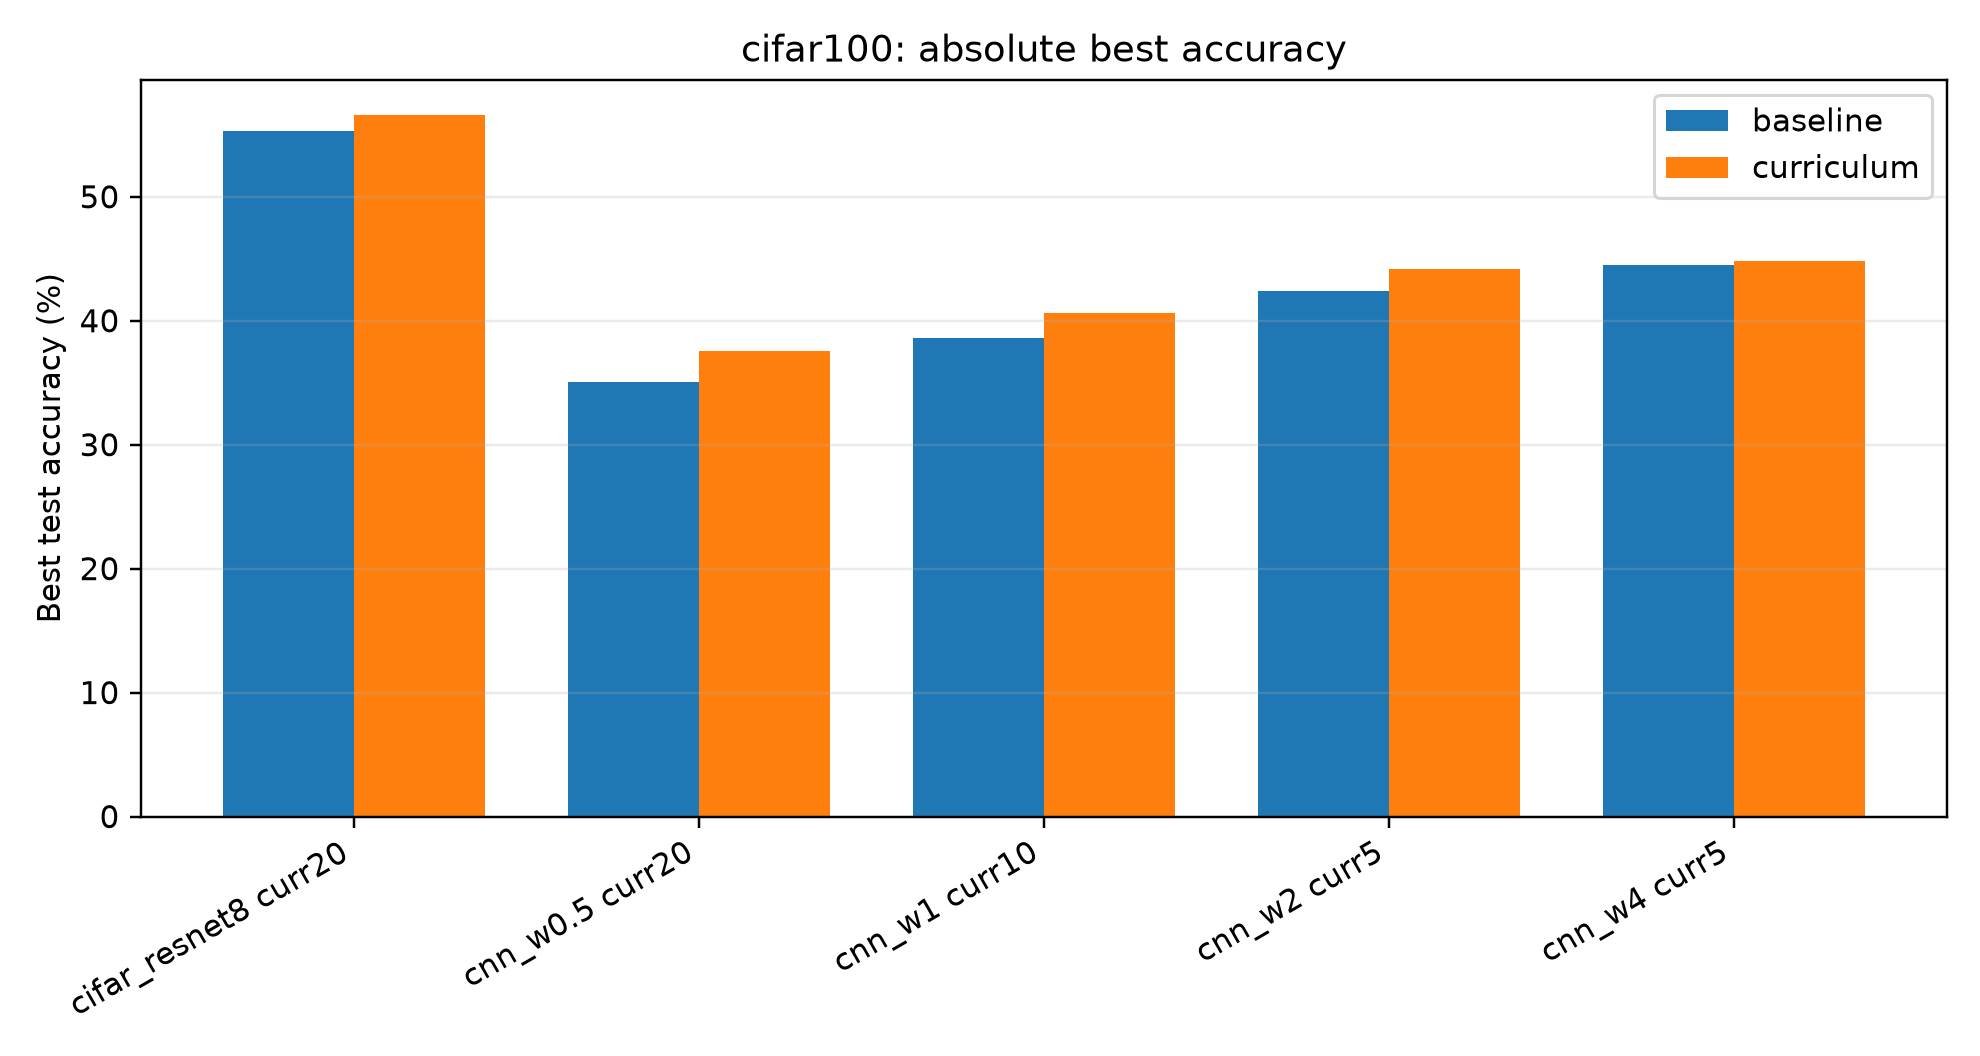
\includegraphics[width=0.82\textwidth]{figures/roughness_followup_updated_cifar100_absolute_best_acc.png}
    \caption{CIFAR-100 absolute best test accuracy for baseline and curriculum
    runs in the updated follow-up.}
    \label{fig:roughness-updated-cifar100-absolute}
\end{figure}

\begin{figure}[h]
    \centering
    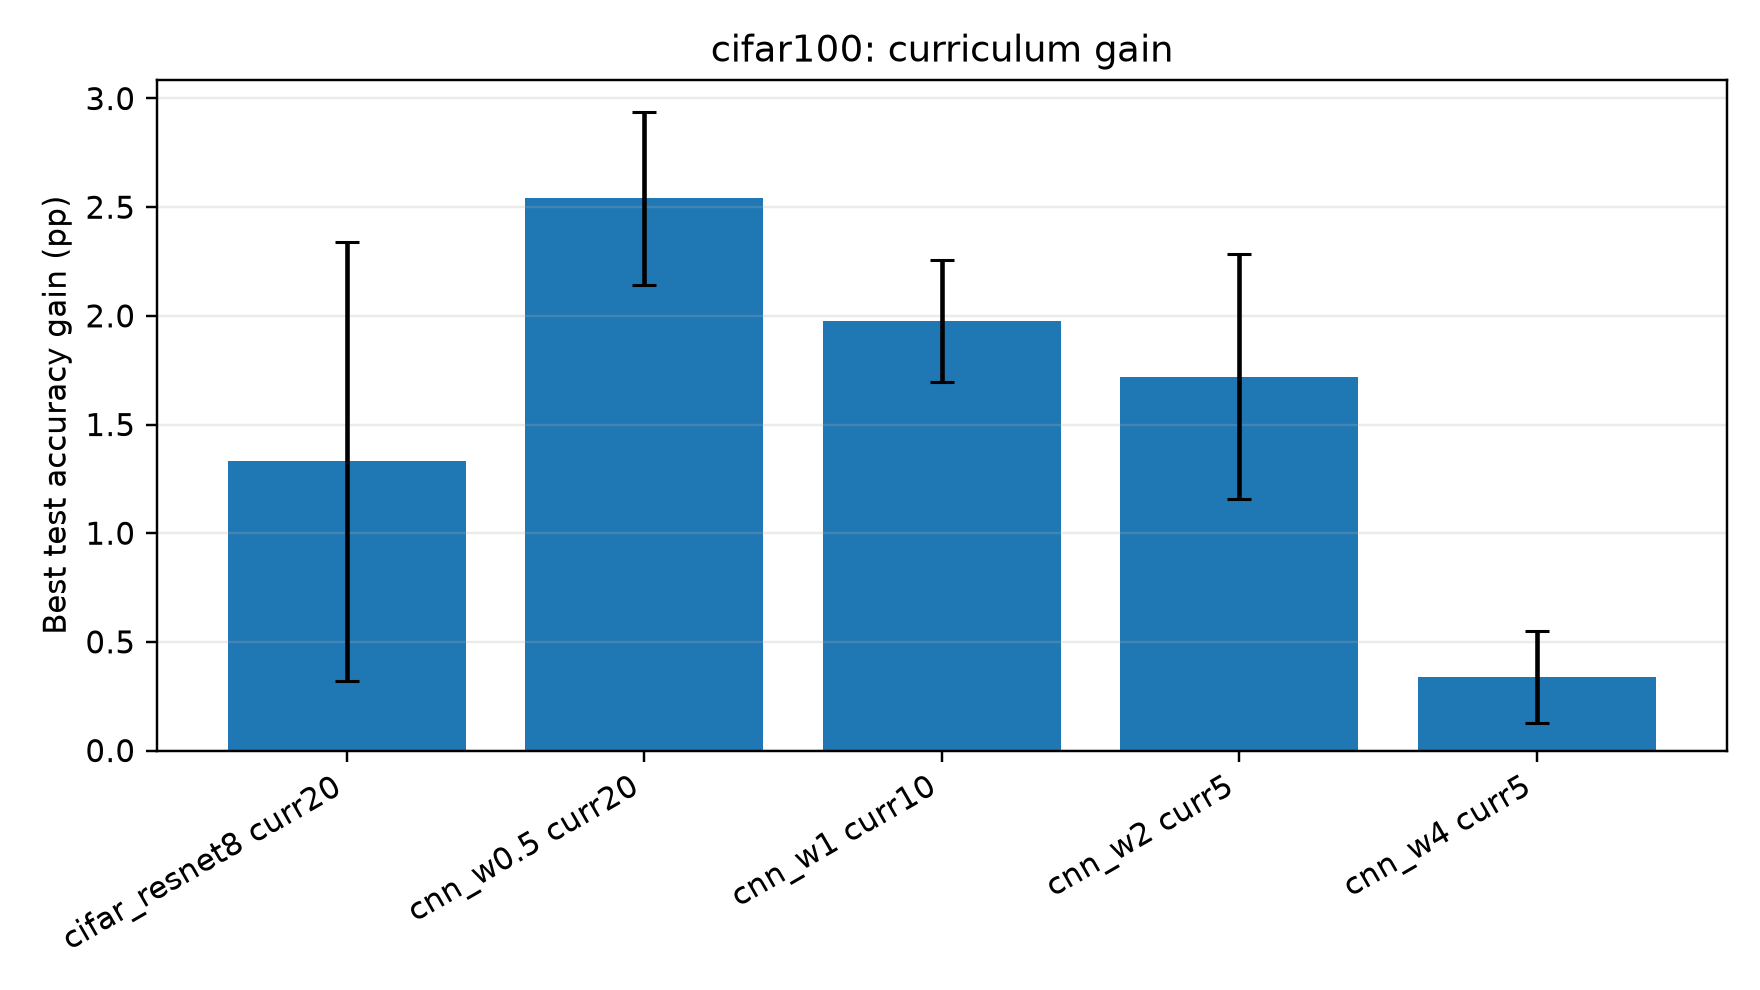
\includegraphics[width=0.82\textwidth]{figures/roughness_followup_updated_cifar100_best_acc_gains.png}
    \caption{CIFAR-100 curriculum gains in best test accuracy. Error bars show
    variation across seeds.}
    \label{fig:roughness-updated-cifar100-gains}
\end{figure}

A subtle point is that \texttt{cnn\_w0.5} improves strongly in best accuracy, but
its final epoch accuracy is almost unchanged. This means the weak CNN overfits or
drifts late in training. For this reason, best accuracy and AUC should both be
reported: curriculum can improve the best solution encountered while still
hurting the average trajectory.

\section{Fashion-MNIST control}

Fashion-MNIST was used as an easy 10-class control. The updated runs include the
original model set and an additional \texttt{cnn\_w0.5} follow-up with
\texttt{curr10} and \texttt{curr20}. Results are shown in
Table~\ref{tab:roughness-fashionmnist-updated}.

\begin{table}[h]
\centering
\small
\begin{tabular}{lrrrrr}
\hline
Model & Curriculum & Base best & Curr best & Gain & AUC gain \\
\hline
\texttt{cnn\_w0.5} & \texttt{curr10} & 0.9066 & 0.9077 & +0.11 & -5.91 \\
\texttt{cnn\_w0.5} & \texttt{curr20} & 0.9066 & 0.9078 & +0.12 & -12.01 \\
\texttt{cnn\_w1} & \texttt{curr10} & 0.9117 & 0.9129 & +0.12 & -6.45 \\
\texttt{cnn\_w4} & \texttt{curr5} & 0.9163 & 0.9148 & -0.16 & -3.25 \\
\texttt{cifar\_resnet8} & \texttt{curr10} & 0.9166 & 0.9124 & -0.42 & -7.43 \\
\hline
\end{tabular}
\caption{Fashion-MNIST updated control results. Absolute best test accuracies
are means over seeds 42, 43, and 44.}
\label{tab:roughness-fashionmnist-updated}
\end{table}

The Fashion-MNIST control is essentially negative. Even the weak
\texttt{cnn\_w0.5} gains only about 0.1 percentage points in best accuracy, while
AUC becomes substantially worse. This supports the interpretation that hard
coarse-to-fine curriculum is not useful simply because a model is small. The task
also needs to be hard enough, and the hierarchy needs to provide meaningful
intermediate supervision.

\begin{figure}[h]
    \centering
    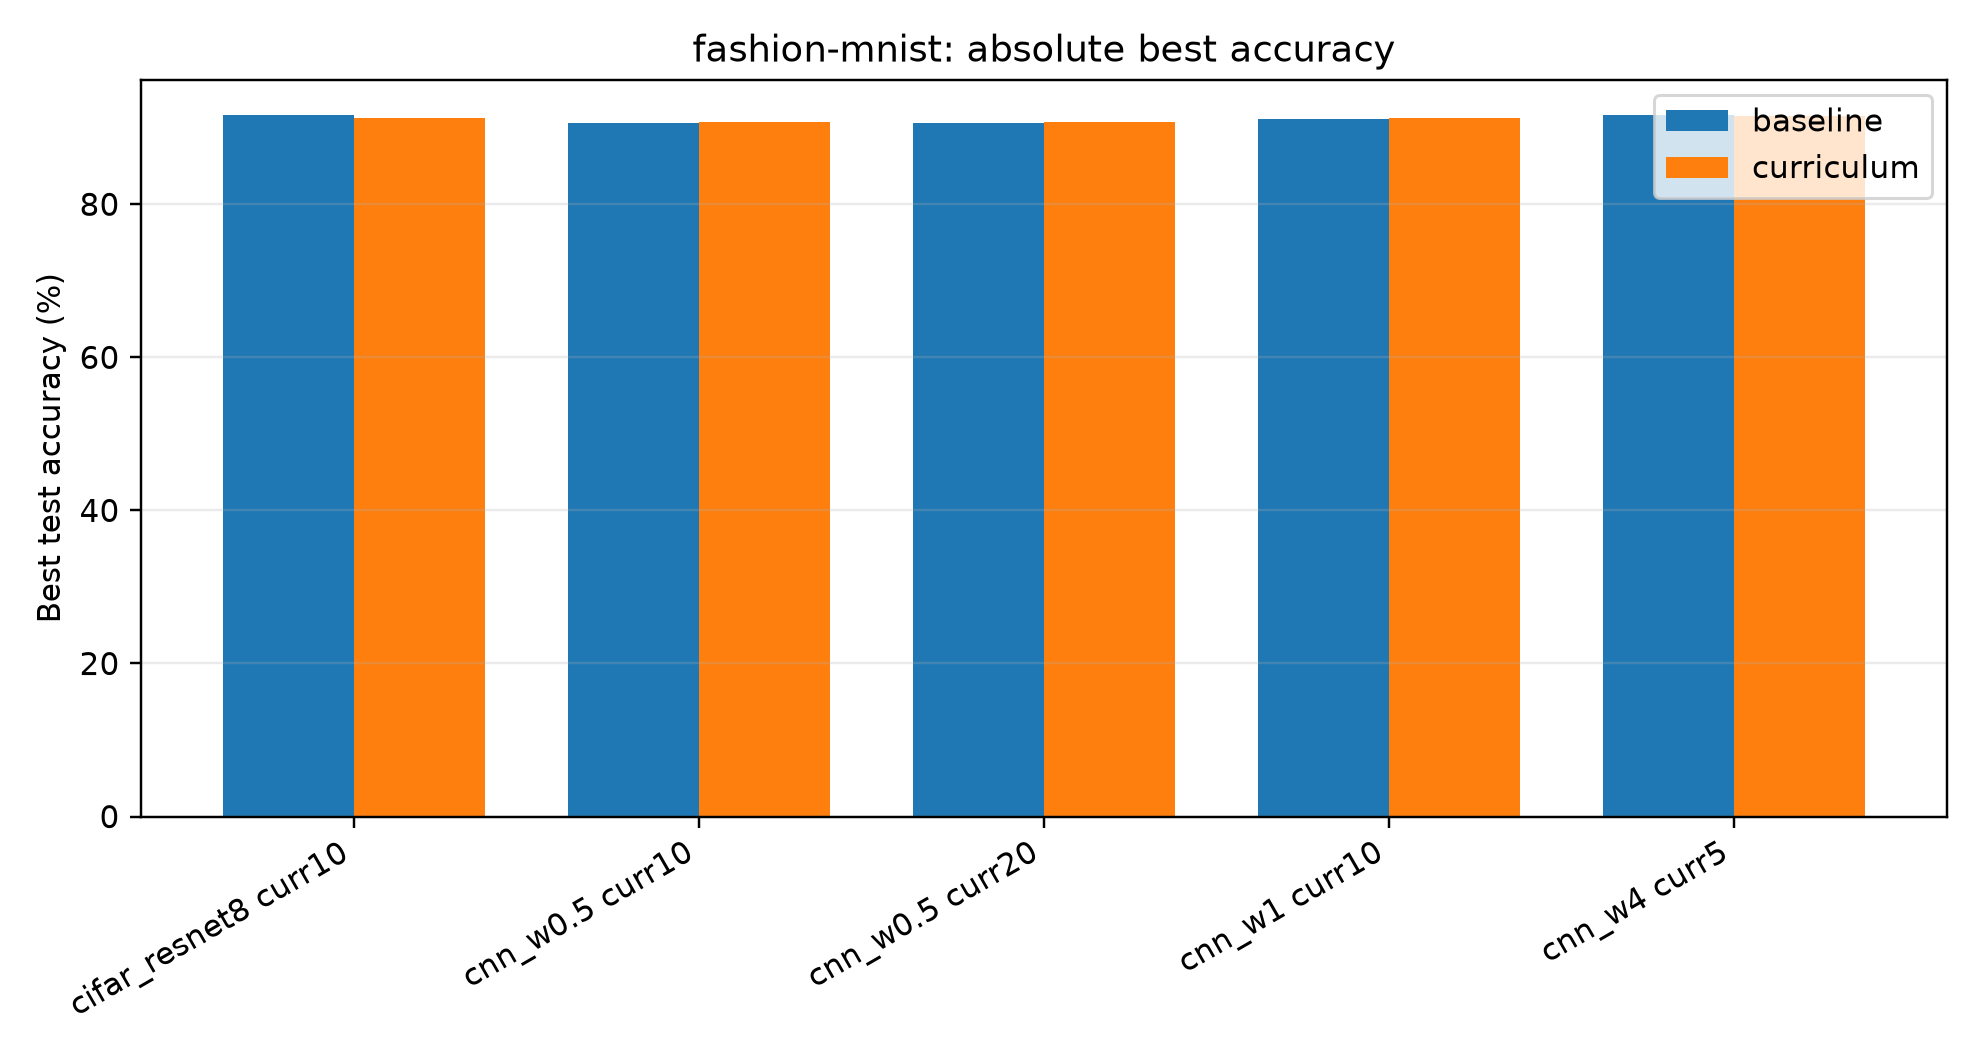
\includegraphics[width=0.82\textwidth]{figures/roughness_followup_updated_fashionmnist_absolute_best_acc.png}
    \caption{Fashion-MNIST absolute best test accuracy. Baselines are already
    high, and curriculum does not add meaningful benefit.}
    \label{fig:roughness-updated-fashionmnist-absolute}
\end{figure}

\section{CIFAR-10 control}

CIFAR-10 was added as a natural-image 10-class control. Unlike Fashion-MNIST, it
shares the image domain of CIFAR-100, but the class count is much smaller and the
automatically generated hierarchy is necessarily shallow. The tested pairs were
\texttt{cnn\_w0.5}/\texttt{curr10}, \texttt{cnn\_w0.5}/\texttt{curr20}, and
\texttt{cifar\_resnet8}/\texttt{curr10}. Results are shown in
Table~\ref{tab:roughness-cifar10-results}.

\begin{table}[h]
\centering
\small
\begin{tabular}{lrrrrr}
\hline
Model & Curriculum & Base best & Curr best & Gain & AUC gain \\
\hline
\texttt{cnn\_w0.5} & \texttt{curr10} & 0.6964 & 0.6988 & +0.24 & -2.80 \\
\texttt{cnn\_w0.5} & \texttt{curr20} & 0.6964 & 0.7042 & +0.78 & -6.75 \\
\texttt{cifar\_resnet8} & \texttt{curr10} & 0.8427 & 0.8436 & +0.09 & -3.61 \\
\hline
\end{tabular}
\caption{CIFAR-10 control results. Absolute best test accuracies are means over
seeds 42, 43, and 44.}
\label{tab:roughness-cifar10-results}
\end{table}

CIFAR-10 gives a small positive result for the weakest CNN, especially for
\texttt{curr20}, but the improvement is much smaller than on CIFAR-100 and comes
with a large AUC penalty. The CIFAR ResNet result is essentially neutral. This
places CIFAR-10 between CIFAR-100 and Fashion-MNIST: there is a small possible
benefit for a weak natural-image CNN, but the effect is not large enough to
change the main conclusion.

\begin{figure}[h]
    \centering
    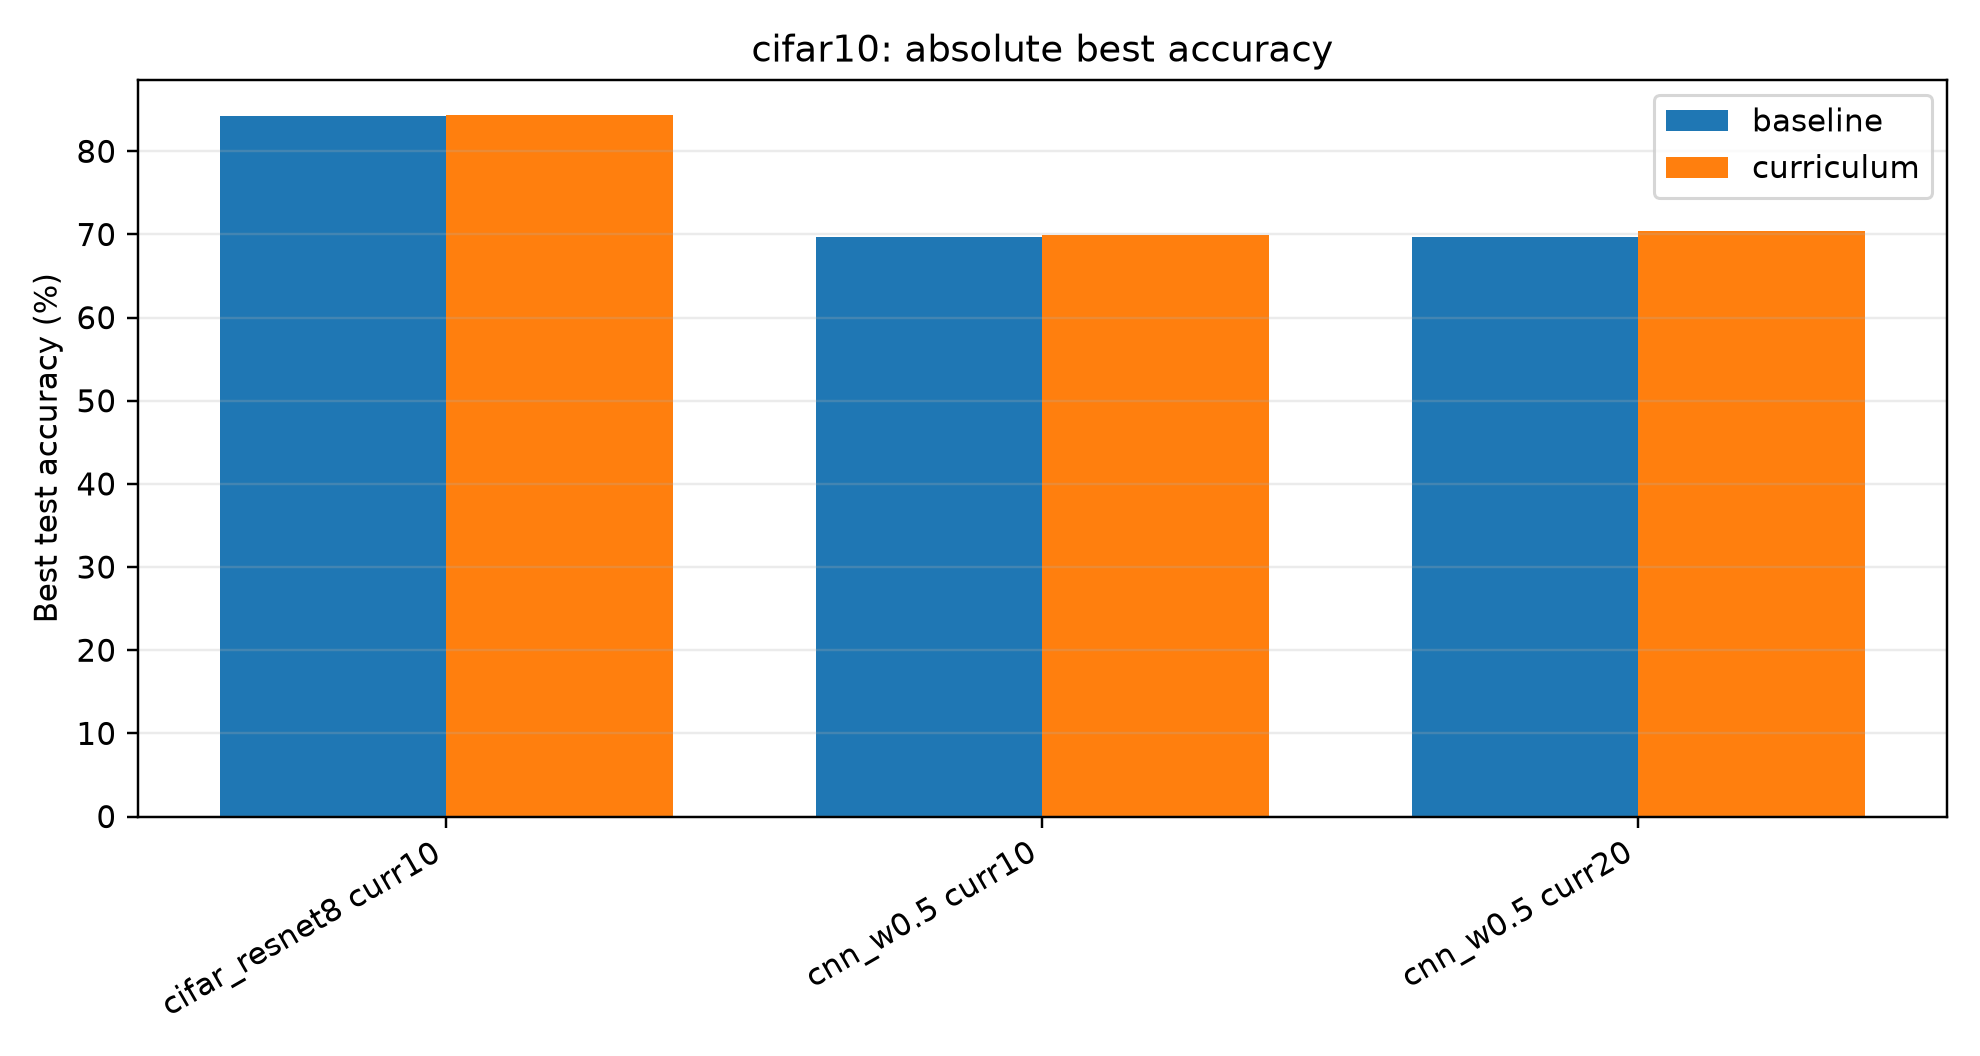
\includegraphics[width=0.82\textwidth]{figures/roughness_followup_updated_cifar10_absolute_best_acc.png}
    \caption{CIFAR-10 absolute best test accuracy for baseline and curriculum
    runs.}
    \label{fig:roughness-updated-cifar10-absolute}
\end{figure}

\begin{figure}[h]
    \centering
    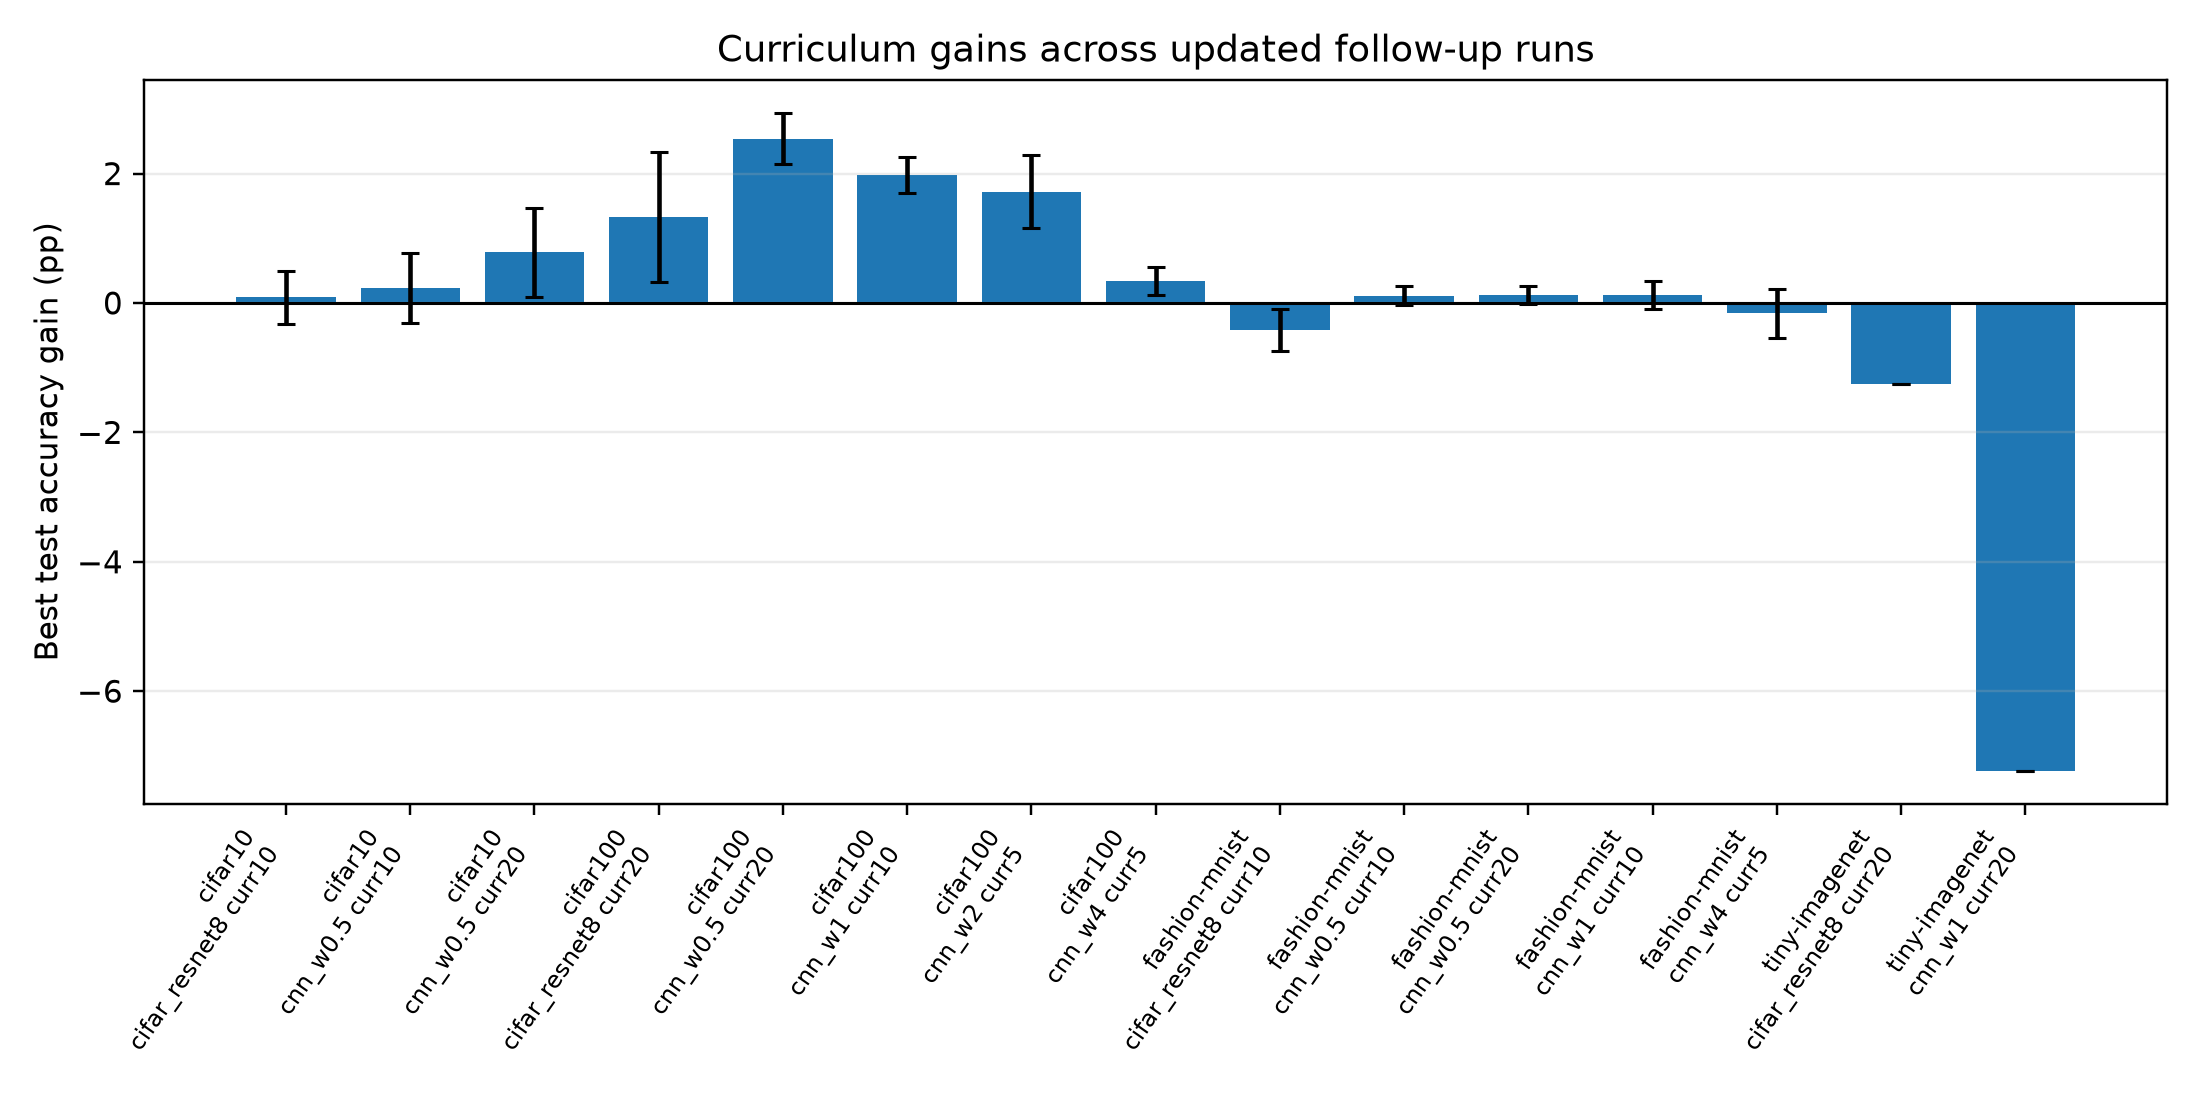
\includegraphics[width=0.95\textwidth]{figures/roughness_followup_updated_all_datasets_best_acc_gains.png}
    \caption{Updated best-test-accuracy gains across CIFAR-100, Fashion-MNIST,
    CIFAR-10, and the Tiny ImageNet pilot.}
    \label{fig:roughness-updated-all-gains}
\end{figure}

\section{Tiny ImageNet pilot}

The minimal Tiny ImageNet pilot used one seed and the pairs
\texttt{cnn\_w1}/\texttt{curr20} and \texttt{cifar\_resnet8}/\texttt{curr20}.
The results are shown in Table~\ref{tab:roughness-tinyimagenet-results}.

\begin{table}[h]
\centering
\small
\begin{tabular}{lrrrrr}
\hline
Model & Curriculum & Base best & Curr best & Gain & AUC gain \\
\hline
\texttt{cnn\_w1} & \texttt{curr20} & 0.2498 & 0.1775 & -7.23 & -5.71 \\
\texttt{cifar\_resnet8} & \texttt{curr20} & 0.3842 & 0.3716 & -1.26 & -5.52 \\
\hline
\end{tabular}
\caption{Tiny ImageNet pilot results. These are one-seed results and should be
interpreted as a stress test rather than a definitive dataset-level conclusion.}
\label{tab:roughness-tinyimagenet-results}
\end{table}

This pilot does not support direct transfer of the CIFAR-100 schedule. The
curriculum hurts both tested models. The most likely explanations are that these
models are too weak for Tiny ImageNet, the generated hierarchy is not good
enough, the curriculum is too long or too hard, or the optimizer/schedule needs
separate tuning. These results should therefore be reported as a negative pilot,
not as a final statement about Tiny ImageNet.

\section{Roughness and sharpness diagnostics}

Table~\ref{tab:roughness-ratios-updated} summarizes selected roughness ratios.
The values are \(\log_{10}(\text{curriculum}/\text{baseline})\), so negative
values mean lower roughness under curriculum and positive values mean higher
roughness.

\begin{table}[h]
\centering
\small
\begin{tabular}{llrr}
\hline
Dataset & Model/curriculum & Final sharp. & Final Hess. \\
\hline
CIFAR-100 & \texttt{cnn\_w0.5}/\texttt{curr20} & +0.03 & +0.03 \\
CIFAR-100 & \texttt{cnn\_w1}/\texttt{curr10} & +0.35 & +0.04 \\
CIFAR-100 & \texttt{cnn\_w2}/\texttt{curr5} & -0.08 & +0.06 \\
CIFAR-100 & \texttt{cnn\_w4}/\texttt{curr5} & +0.15 & +0.23 \\
CIFAR-100 & \texttt{cifar\_resnet8}/\texttt{curr20} & -0.16 & -0.30 \\
Fashion-MNIST & \texttt{cnn\_w0.5}/\texttt{curr20} & -0.10 & -0.41 \\
CIFAR-10 & \texttt{cnn\_w0.5}/\texttt{curr20} & +0.12 & +0.19 \\
Tiny ImageNet & \texttt{cnn\_w1}/\texttt{curr20} & +0.08 & +0.20 \\
\hline
\end{tabular}
\caption{Selected roughness log-ratios. Negative values indicate lower final
roughness under curriculum.}
\label{tab:roughness-ratios-updated}
\end{table}

The roughness results remain mixed after the added runs. The cleanest support
for a flattening interpretation is still CIFAR-100 \texttt{cifar\_resnet8}, where
curriculum improves accuracy and lowers both final sharpness and Hessian
estimates. The CNNs do not show a universal pattern. For example,
\texttt{cnn\_w0.5} and \texttt{cnn\_w1} improve on CIFAR-100, but their final
roughness is not consistently lower. This means the thesis should not claim that
coarse-to-fine curriculum works by always finding flatter minima.

The safer interpretation is that curriculum changes the optimization trajectory
and can improve the best solution found for some lower-capacity models. The
roughness probes are useful diagnostics, but they do not yet identify one simple
causal mechanism.

\section{Learned hierarchy inspection}

The new runs save a readable hierarchy file, \texttt{hierarchy.md}, as a W\&B
artifact. For example, a Fashion-MNIST curriculum run stores the generated
clusters under a path like:

\begin{verbatim}
/runpod-workspace/runs/<run_id>/fashion-mnist_cnn_curriculum/hierarchy.md
\end{verbatim}

and uploads the same file to W\&B artifacts. The same files were also exported
locally under:

\begin{verbatim}
thesis/appendices/hierarchies/
\end{verbatim}

The hierarchy is generated from the baseline classifier-weight distance matrix,
not from official semantic labels. Therefore it should be interpreted as the
model's learned similarity structure, rather than as a ground-truth taxonomy.
Tables~\ref{tab:hier-fashionmnist}, \ref{tab:hier-cifar10-cnn}, and
\ref{tab:hier-cifar10-resnet8} show representative learned hierarchies from seed
42. For these 10-class datasets the hierarchy has only one non-trivial coarse
level plus the singleton fine-label level.

\begin{table}[h]
\centering
\small
\begin{tabular}{lp{0.72\textwidth}}
\hline
Cluster & Fashion-MNIST \texttt{cnn\_w0.5}, seed 42, \texttt{curr20} \\
\hline
1 & \texttt{t-shirt\_top}, \texttt{trouser}, \texttt{coat}, \texttt{sandal}, \texttt{bag} \\
2 & \texttt{pullover}, \texttt{shirt}, \texttt{sneaker} \\
3 & \texttt{ankle\_boot}, \texttt{dress} \\
\hline
\end{tabular}
\caption{Representative Fashion-MNIST learned hierarchy. The grouping is only
partly semantic, which helps explain why curriculum did not provide a meaningful
benefit on this dataset.}
\label{tab:hier-fashionmnist}
\end{table}

\begin{table}[h]
\centering
\small
\begin{tabular}{lp{0.72\textwidth}}
\hline
Cluster & CIFAR-10 \texttt{cnn\_w0.5}, seed 42, \texttt{curr20} \\
\hline
1 & \texttt{airplane}, \texttt{bird}, \texttt{deer}, \texttt{horse}, \texttt{ship} \\
2 & \texttt{automobile}, \texttt{truck} \\
3 & \texttt{cat}, \texttt{dog}, \texttt{frog} \\
\hline
\end{tabular}
\caption{Representative CIFAR-10 hierarchy learned from a weak CNN baseline.
Some clusters are intuitive, for example vehicles and animals, but the hierarchy
is necessarily shallow because CIFAR-10 has only ten classes.}
\label{tab:hier-cifar10-cnn}
\end{table}

\begin{table}[h]
\centering
\small
\begin{tabular}{lp{0.72\textwidth}}
\hline
Cluster & CIFAR-10 \texttt{cifar\_resnet8}, seed 42, \texttt{curr10} \\
\hline
1 & \texttt{airplane}, \texttt{bird}, \texttt{deer} \\
2 & \texttt{ship}, \texttt{automobile}, \texttt{truck}, \texttt{frog} \\
3 & \texttt{cat}, \texttt{dog}, \texttt{horse} \\
\hline
\end{tabular}
\caption{Representative CIFAR-10 hierarchy learned from a CIFAR-style ResNet-8
baseline. The grouping differs from the CNN hierarchy, showing that the
curriculum depends on the reference model as well as the dataset.}
\label{tab:hier-cifar10-resnet8}
\end{table}

For CIFAR-100 the hierarchy is too large to print in full, but the top level of
the \texttt{cnn\_w0.5}, seed 42 hierarchy is shown in
Table~\ref{tab:hier-cifar100-top}. The complete exported Markdown and JSON files
are included in \texttt{thesis/appendices/hierarchies/}.

\begin{table}[h]
\centering
\scriptsize
\begin{tabular}{lp{0.78\textwidth}}
\hline
Cluster & CIFAR-100 top-level classes, \texttt{cnn\_w0.5}, seed 42, \texttt{curr20} \\
\hline
1 & \texttt{apple}, \texttt{sweet\_pepper}, \texttt{orange}, \texttt{pear}, \texttt{butterfly}, \texttt{possum}, \texttt{squirrel} \\
2 & \texttt{aquarium\_fish}, \texttt{train}, \texttt{lawn\_mower}, \texttt{bridge}, \texttt{bus}, \texttt{lobster}, \texttt{skyscraper}, \texttt{streetcar}, \texttt{chair}, \texttt{chimpanzee}, \texttt{cloud}, \texttt{tractor}, \texttt{pickup\_truck}, \texttt{willow\_tree}, \texttt{forest}, \texttt{rocket}, \texttt{keyboard}, \texttt{maple\_tree}, \texttt{spider}, \texttt{oak\_tree}, \texttt{tank}, \texttt{palm\_tree}, \texttt{pine\_tree}, \texttt{shark}, \texttt{bed}, \texttt{couch}, \texttt{plain}, \texttt{road}, \texttt{sea}, \texttt{castle}, \texttt{house}, \texttt{mountain} \\
3 & \texttt{lamp}, \texttt{cup}, \texttt{telephone}, \texttt{baby}, \texttt{girl}, \texttt{woman}, \texttt{boy}, \texttt{man}, \texttt{rose}, \texttt{caterpillar}, \texttt{orchid} \\
4 & \texttt{mouse}, \texttt{shrew}, \texttt{otter}, \texttt{wolf}, \texttt{raccoon}, \texttt{bear}, \texttt{seal}, \texttt{tiger}, \texttt{skunk}, \texttt{porcupine}, \texttt{elephant}, \texttt{mushroom}, \texttt{snail}, \texttt{sunflower}, \texttt{bee}, \texttt{tulip}, \texttt{dinosaur}, \texttt{poppy}, \texttt{rabbit}, \texttt{bottle}, \texttt{fox}, \texttt{hamster}, \texttt{cattle}, \texttt{camel} \\
5 & \texttt{leopard}, \texttt{lion}, \texttt{trout}, \texttt{crocodile}, \texttt{beaver}, \texttt{ray}, \texttt{turtle}, \texttt{bicycle}, \texttt{motorcycle}, \texttt{lizard}, \texttt{kangaroo}, \texttt{cockroach}, \texttt{flatfish}, \texttt{dolphin}, \texttt{whale} \\
6 & \texttt{worm}, \texttt{snake}, \texttt{can}, \texttt{table}, \texttt{television}, \texttt{bowl}, \texttt{wardrobe}, \texttt{plate}, \texttt{clock}, \texttt{crab}, \texttt{beetle} \\
\hline
\end{tabular}
\caption{Top level of the representative CIFAR-100 learned hierarchy. The
clusters contain a mixture of semantic and visually learned associations, which
is expected because the hierarchy is derived from classifier weights rather than
human labels.}
\label{tab:hier-cifar100-top}
\end{table}

This qualitative inspection is important because it separates two possible
failure modes: curriculum may fail because coarse labels are not useful for a
particular model, or because the generated hierarchy itself is poor. This
distinction is especially relevant for Tiny ImageNet, where the negative pilot
may reflect hierarchy quality, model capacity, or schedule choice rather than the
absence of any useful class structure.

\section{Interpretation}

The updated follow-up supports the following thesis-level conclusions.

First, CIFAR-100 remains the strongest positive case. The added
\texttt{cnn\_w0.5} runs show the largest gain in the follow-up, which reinforces
the capacity-conditioned result: the weaker CNNs benefit most from curriculum.

Second, the effect does not transfer automatically to easy 10-class datasets.
Fashion-MNIST is essentially negative, and CIFAR-10 shows only a small gain for
\texttt{cnn\_w0.5}. This suggests that both model weakness and dataset structure
matter. A weak model alone is not sufficient.

Third, the Tiny ImageNet pilot is negative under the tested settings. It should
not be used to conclude that curriculum cannot work on Tiny ImageNet, but it does
show that the CIFAR-100 schedule and generated hierarchy are not directly
plug-and-play.

Fourth, roughness and sharpness diagnostics are inconclusive as a mechanism.
Some successful curriculum runs are flatter by these probes, while others are
not. Therefore the correct claim is:

\begin{quote}
The experiments confirm a capacity- and dataset-dependent curriculum effect, but
current roughness probes do not prove that this effect is caused by consistently
finding flatter minima.
\end{quote}

This is the most defensible interpretation for the final thesis.
